\documentclass[12pt]{report}
%\usepackage{aums}       % For Master's papers
\usepackage{auphd}     % For Ph.D.
%\usepackage{auhonors}  % For honors college
%\usepackage{ulem}       % underlining on style-page; see \normalem below
%\usepackage{url}
%\usepackage{tikz}
%\usepackage{pgf}

%% If you do not need a List of Abbreviations, then comment out the lines below and the \printnomenclature line.
%%for List of Abbreviations information:  (see http://www.mackichan.com/TECHTALK/509.htm  )
\usepackage[intoc]{nomencl}
\renewcommand{\nomname}{List of Abbreviations}   	       
\makenomenclature 
%% don't forget to run:   makeindex ausample.nlo -s nomencl.ist -o ausample.nls
%% Also, if 
%\usepackage{chapterbib}

\usepackage{algorithm}
\usepackage{algorithmic}
\usepackage{amsmath}
\usepackage{amssymb}
\usepackage{caption}
\usepackage{amsthm}
\usepackage{chapterbib}
\usepackage{color}
\usepackage{cite,float}
\usepackage{epsfig}
\usepackage{flushend}
\usepackage{graphicx}
\usepackage{import}
\usepackage{listings}
\usepackage{multirow}
\usepackage{paralist}
\usepackage{setspace}
\usepackage{subfigure}
\usepackage{times}
\usepackage{upquote}
\usepackage{verbatim}

%\newtheorem{theorem}{Theorem}
\newtheorem{lemma}{Lemma}[section]
\newtheorem{axiom}{Axiom}
\newtheorem{property}{Property}[section]
%\newtheorem{proposition}[theorem]{Proposition}
\newtheorem{definition}{Definition}[section]

% May want theorems numbered by chapter
\newtheorem{theorem}{Theorem}[chapter]

%\renewcommand{\nomname}{List of Abbreviations}

\newenvironment{remark}[1][Remark]{\begin{trivlist}\item[\hskip \labelsep {\bfseries #1}]}{\end{trivlist}}

%%
% Define code listing style. This is used in conjunction with caption style defined below.
%%
\lstset{
    %basicstyle=\small\ttfamily,
    basicstyle=\ttfamily,
    numbers=left,
    %numberstyle=\tiny,
    %stepnumber=2,
    %numbersep=8pt,
    tabsize=2,
    %extendedchars=true,
    breaklines=true,
%    keywordstyle=\color[rgb]{0.12, 0.2, 0.40},
%    commentstyle=\color[rgb]{0.4,0.4,0.4},
%    stringstyle=\color[rgb]{0,0.5,0.51},
%    identifierstyle=\color[rgb]{0.8,0.09,0.43},
	frame=tb,         
    %captionpos=t,
    %keywordstyle=[1]\textbf,
    %keywordstyle=[2]\textbf,
    %keywordstyle=[3]\textbf,
    %keywordstyle=[4]\textbf,
    showspaces=false,
    showtabs=false,
    xleftmargin=20pt,
    framexleftmargin=20pt,
    %framexrightmargin=5pt,
    %framexbottommargin=4pt,
    %backgroundcolor=\color{lightgray},
    showstringspaces=false 
}

%%
% A listing style for Java code.
%%
\lstdefinestyle{java}{
    identifierstyle=\color{black},
}
  
%%
% A listing style that is currently not used.
%%
\lstdefinestyle{test}{
    basicstyle=\small\ttfamily,
    identifierstyle=\color{black},
    %belowcaptionskip=1\baselineskip,
    breaklines=true,
    frame=l,
    language=sql,
    numbers=left,
    xleftmargin=\parindent,
    %showstringspaces=false,
    %keywordstyle=\bfseries\color{green!40!black},
    %commentstyle=\itshape\color{purple!40!black},
    %identifierstyle=\color{blue},
    %stringstyle=\color{orange},
}

\def\inline{\lstinline[basicstyle=\small\ttfamily,identifierstyle=\color{green}]}

%% 
% Define Style to gray background and white text.
%%
%\DeclareCaptionFont{white}{\color{white}}
%\DeclareCaptionFormat{listing}{\colorbox[cmyk]{0.43, 0.35, 0.35,0.01}{\parbox{\columnwidth}{#1#2#3}}}
%\captionsetup[lstlisting]{format=listing,labelfont=white,textfont=white, singlelinecheck=false, margin=0pt, font={bf,footnotesize}}

\author{Chih Jye Wang}
\date{November 20, 2015} %date of graduation
\copyrightyear{2015} %copyright year

\keywords{Database management systems, R-Tree index, skyline computation, index-based pruning skyline, hierarchical relational database, SPARQL, spatial SPARQL, fusion experiments, control systems, MDPX}

% Put the Thesis Adviser here.
\adviser{Wei-Shinn Ku}


% Put the committee here (including the adviser), one \professor for each.
% The advisor must be first, and the dean of the graduate school must be last.
\professor{Wei-Shinn Ku, Chair, Associate Professor of Computer Science and Software Engineering}
\professor{Xiao Qin, Professor Computer Science and Software Engineering}
\professor{James Cross, Professor of Computer Science and Software Engineering}
\professor{Alvin Lim, Professor of Computer Science and Software Engineering}
\professor{Edward Thomas, Jr., Professor Physics}


%\title{Index for Relational Hierarchical Structures and A Case Study of Migration from MySQL to MongoDB (Draft)}
%\title{Hierarchical and Spatial Indexing in Scientific Database}
\title{Index Structures for Hierarchical, Spatial, and Unstructured Data in Scientific and Dusty Plasma Physics Database}

\begin{document}

\begin{romanpages}      % roman-numbered pages 

\TitlePage 

\begin{abstract}
This presentation presents the computerized control and data acquisition and management system for the Magnetized Dusty Plasma Experiment (MDPX), which was commissioned in Fall of 2014 at Plasma Physics Laboratory at Auburn University. The purpose of this new device is to study behavior and phenomenons of electrically-charged dust particulates in plasma under high uniform or gradient magnetic field. The control system is a customized interface running LabView software. Hardware devices are interfaced with the control system via National Instrument PXIe-1075 PXI Express chassis. A file-based hierarchy structure is used to store research data obtain from diagnostic hardware during experiments. The hierarchical structure allows the storage of heterogeneous of data formats from various hardware systems. A relational database is used to index and retrieval research data.

Two relational model structures and data retrieval techniques are studied and optimized. Due to the hierarchical structure of the MDPX data, it is the first structure studied. Data in relational model is divided into flat tables and ineffective for representing hierarchical data. We designed an index for hierarchical model using the nested sets technique. We compare the performance of our design using adjacency list, stored procedure, and nested sets methods. Evaluation indicates our approach improves the data retrieval rate for many operations.

The second technique we study is to retrieve best data across multiple attributes from a database based on user search criteria, also know as skyline. Existing techniques of skyline evaluation only considering minimizing attributes and only consider data of two dimensions. In our study, we propose a novel way to evaluate skyline using non-overlapping spatial index. The technique allows user to specify either to minimize or maximizing data attributes of arbitrary data dimensions. The non-overlapping feature of our technique allows it to perform better than best-first-search (BFS) algorithm.

%Computer databases are ubiquitous and play an important role in most software projects. Although database systems has been used for more than five decades, there are still challenges to be solved. This study is composed of three parts. The first part studies hierarchical data in relational database and proposes an index to facilitate query evaluation. The second part details an index and algorithm for evaluating skyline operation in database. Final and the third part explorers the advantages and disadvantages of moving from relational database to semantic web data model using RDF.
\end{abstract}

%\begin{acknowledgments}
%Put text of the acknowledgments here.
%\end{acknowledgments}

\tableofcontents
\listoffigures
\listoftables
%\printnomenclature[0.5in] %used for the List of Abbreviations
\end{romanpages}        % All done with roman-numbered pages


%\normalem       % Make italics the default for \em

\chapter{Efficient Evaluation of Skyline Queries in Wireless Data Broadcast Environments}
\import{bsky/}{BSky}

\chapter{Computerized Control and Data Acquisition System for MDPX}
\import{mdpx/}{body}

\chapter{Hierarchical Data in Relational Database Management Systems}
\import{reltree-paper/text/}{body}

%\chapter{A Case Study of Migration from MySQL to MongoDB}
%\import{mongodb/}{body}

\chapter{Geo-Store: A Spatially-Aware SPARQL Evaluation Engine}

%\begin{abstract}
%
Today, location-based services (LBS) are very popular information
services for mobile users who access the services with
location-aware mobile devices through wireless networks. The data
sources of advanced LBSs are on the Web, which consists of a huge
volume of data in human-readable format. The main goal of the
Semantic Web is to augment the Web with information so that
computers can understand and exchange Web data. Therefore, it will
be a trend for LBS providers to employ Semantic Web data sources
to develop semantics-enabled location-based services. However,
there are currently limited solutions to process spatial queries,
the building blocks of most LBSs, on Semantic Web data for
supporting location-based services. This article describes our
novel spatial query techniques, which are able to efficiently
evaluate spatial queries on RDF triple stores (Semantic Web data
management systems) for providing semantics-enabled location-based
services.

%\end{abstract}

\section{Introduction}\label{sec-intro}

With the popularity of wireless networks and mobile devices,
Location-Based Services (LBS) have become indispensable
applications to mobile users. The global GPS navigation and LBS
market size has been predicted to grow significantly from \$1.6
billion in 2009 to \$13.4 billion in 2014 according to IEMR's
report ``Global GPS Navigation and Location Based Services
Forecast". In addition, the Web consists of a huge volume of data
which requires the use of human intelligence to process and analyze. The main goal of the
Semantic Web is to augment the Web with information so that
computers can understand and exchange Web data. Consequently, it
will be a trend for LBS providers to employ Semantic Web data
sources to develop semantics-enabled location-based services.

The Resource Description Framework (RDF) data model is designed
for interchanging schema-relaxable (or schema-less) data on the
Semantic Web~\cite{RDF}. RDF models the linking structure of the
Web as triples of the form $\langle s, p, o \rangle$, where $s$ is
a subject, $p$ is a predicate, and $o$ is an object. Each triple
represents the relationship between the subject and the object. A
collection of triples forms a directed graph, where the edges
represent predicates between subjects and objects, which are
represented by the graph nodes. With the increasing amount of RDF
data on the Web, researchers developed specialized architectures
for RDF data management named \emph{triple
stores}~\cite{conf/www/CarrollDDRSW04,conf/vldb/ChongDES05,conf/vldb/AbadiMMH07,
journals/pvldb/WeissKB08,journals/vldb/NeumannW10}. Generally,
these solutions employ various indexing, compression, and query
optimization techniques for scalable and efficient management of
RDF data.

The Semantic Web is an ideal data source for supporting the
state-of-the-art location-based services that employ dynamic or
near real-time information. For example, a mobile user may utilize
LBS to search for nearby restaurants based on recent reviews on
the Web. However, to the best of our knowledge, there are limited
solutions to process spatial queries, the building blocks of most
LBSs, on triple stores for supporting advanced location-based
services. Therefore, the goal of the Geo-Store project is to
develop novel spatial query techniques that are able to
efficiently evaluate spatial queries on RDF triple stores for
providing semantics-enabled location-based services. The main
features of our Geo-Store system are as follows.

\begin{itemize}
    \item The Geo-Store system employs a novel representation to
    model spatial features and utilizes a spatial mapping
    mechanism to preserve spatial locality.\vspace*{-3pt}

    \item The Geo-Store system is able to effectively process both range and $k$ Nearest Neighbor ($k$NN)
    queries, the building blocks of many LBS applications, on RDF triple stores.\vspace*{-3pt}

    \item Users are able to integrate and operate the Geo-Store system on
    existing triple stores (e.g., RDF-3X) with limited changes.\vspace*{-3pt}
\end{itemize}


\section{Related Work}\label{sec-relwork}

Location-based services are any service that takes into account
the geographic location of an entity and are accessible with
mobile devices through wireless
networks~\cite{journals/cacm/JunglasW08}. With the prevalence of
GPS-enabled mobile devices and the introduction of 4G mobile
telecommunications services, various commercial LBSs, such as
location-based dating, location-targeted advertisement, and child
safety services, appear in our
lives~\cite{journals/pervasive/BellavistaKH08}. In addition, novel
LBS applications are able to exploit online Semantic Web sources
(e.g., LinkedGeoData\footnote{http://linkedgeodata.org}) about
nearby physical entities of a user to provide personalized
services~\cite{journals/internet/WoenselCPT11}. Today,
location-based services are applied in different fields, such as
emergency response, navigation, product tracking, social networks,
etc.

%The origin of LBS was the Enhanced 911 (E911) mandate which was
%issued by the US Federal Communication Commission (FCC) to improve
%emergency responses to wireless 911 calls by determining a
%caller's location with prescribed accuracy.

%\footnote{http://www.w3.org/standards/semanticweb/}

The Semantic Web is a group of techniques for machines to
understand information and exchange knowledge on the World Wide
Web. The cornerstone of the Semantic Web is a logical data model
named RDF which employs triples to represent the relationships
between subjects and objects. In order to efficiently manage RDF
data, there are numerous systems invented for storing and querying
triple
collections~\cite{conf/www/CarrollDDRSW04,conf/vldb/ChongDES05,conf/vldb/AbadiMMH07,
journals/pvldb/WeissKB08,journals/vldb/NeumannW10}. For improving
performance and scalability, Abadi et
al.~\cite{conf/vldb/AbadiMMH07} introduced a solution by
vertically partitioning the RDF data. Their solution's performance
can be further improved by utilizing a column-oriented DBMS, which
is a database designed specially for the vertically partitioned
case. Weiss et al.~\cite{journals/pvldb/WeissKB08} proposed a
sextuple-indexing scheme, named Hexastore, which allows for quick
and scalable general purpose query evaluation for RDF data
management. Hexastore achieves significant advantages in
performance compared with previous solutions for managing RDF
triples. The RDF-3X engine~\cite{journals/vldb/NeumannW10} is an
implementation of the SPARQL query language~\cite{SPARQL} for RDF
by pursuing a simplified architecture with streamlined indexing
and query processing. The design of RDF-3X completely eliminates
the need for index tuning by exhaustive indexes for all
permutations of subject-predicate-object triples and their binary
and unary projections. However, all the aforementioned triple
stores do not consider the unique features of spatial data when
they encode and store RDF triples.

%In addition, the query processor is able to leverage fast merge
%joins for improving query performance.

Recently, Perry et al.~\cite{Perry11} presented an extension to
SPARQL, named SPARQL-ST, for complex spatiotemporal queries. They
implemented SPARQL-ST by extending a relational database, which is
not an effective way of managing RDF triples. The Strabon system
is an implementation of the data model stRDF and the query
language stSPARQL~\cite{conf/esws/KoubarakisK10}, which are
extensions of RDF and SPARQL for managing spatial and temporal
data. Nevertheless, Strabon is built on top of the RDF store
Sesame\footnote{http://www.openrdf.org/} which is not as efficient
as the aforesaid new generation RDF triple
stores~\cite{KyzirakosKK10}. Brodt et
al.~\cite{conf/gis/BrodtNM10} proposed a solution to integrate
spatial query processing into RDF triple stores. However, their
design cannot efficiently evaluate queries on large-scale spatial
data sets, which are essential for the state-of-the-art LBSs.
Furthermore, Parliament~\cite{conf/SSWS09,conf/semweb/KolasS07} is
a triple store and employs a similar approach
to~\cite{conf/gis/BrodtNM10} for spatial queries and storage of
the data. The GeoSPARQL draft standard~\cite{GeoSPARQL} is
currently being implemented in Parliament.

%Therefore, we need novel techniques to manage spatial RDF data and
%efficiently enable semantics-enhanced location-based services.


\section{The Geo-Store System}\label{sec-design}
Although many RDF triple stores have been proposed during the past few years, most of them were designed and optimized mainly for non-spatial Semantic Web data. In order to enable spatial query processing on RDF triple stores, the state-of-the-art method~\cite{conf/gis/BrodtNM10} is to treat all the Universal Resource Identifiers (URIs) and literals, non-spatial or spatial, equally and replace each URI and literal with an integer ID by dictionary encoding. As a result, each spatial literal (e.g., the latitude and longitude coordinates or the address) is mapped to a randomly generated ID. Afterwards, an R-tree (or its variant)~\cite{reference/gis/HadjieleftheriouMTT08} is created to index all the IDs referred to spatial literals. However, this dictionary encoding-based method may incur extreme inefficiency in evaluating spatial queries on RDF triple stores, especially when coping with large-scale spatial data sets~\cite{conf/gis/BrodtNM10}. In this chapter, we employ a novel representation, \emph{GeoHilbert} -- an RDF vocabulary as an extension of the Geography Markup Language (GML), to model spatial features based on their Hilbert curve~\cite{journals/tkde/MoonJFS01} transformation information and to utilize Spatially Aware Mapping (SAM), instead of dictionary mapping, to encode URIs and literals for preserving spatial locality.

\subsection{Data Representation}

Because many huge data repositories published online contain geographic location or spatial relationship information, we are witnessing a new research trend of modeling geographic entities ontologically and querying their spatial relations in the Semantic Web community. As one of the Semantic Web technologies, the Resource Description Framework treats relationships as first-class citizens and, consequently, can work as an ideal tool for modeling and querying complex and large amounts of relations between spatial entities. The XML formatted semantic data can be converted to the corresponding RDF representation with minor modifications. For example, Listing~\ref{list2} shows an XML data excerpt from the OpenStreetMap project\footnote{http://www.openstreetmap.org/}. This snippet describes the referred information (semantic and spatial) about a restaurant in Pasadena, California, USA. Its corresponding RDF representation is demonstrated in Listing~\ref{list3}. Specifically, \emph{gml} represents the namespace\footnote{http://www.opengis.net/gml} of the GML standard, and \emph{gstore} corresponds to the namespace\footnote{http://example.org/gstore} of our Geo-Store system.

%The RDF data is a collection of RDF triples, and each RDF triple
%is of the form $\langle subject, predicate, object \rangle$, where
%\emph{subject} is the URI of a resource, \emph{predicate}
%represents a particular relationship, and \emph{object} denotes a
%URI of another resource or a literal.

%Table~\ref{tab-prefix} shows the namespace prefixes used in this
%article.

%\lstset{showstringspaces=false} \lstset{basicstyle=\ttfamily\small,escapeinside={`}{`}}

\begin{lstlisting}[caption={An XML data excerpt from the OpenStreetMap project.}, label={list2}]
<node id="738330640" lat="34.1135498" lon="-118.1235345" user="AM909" uid="82317" visible="true" version="1" changeset="4737707" timestamp="2010-05-18T11:26:40Z">
  <tag k="amenity" v="restaurant" />
  <tag k="cuisine" v="american" />
  <tag k="name" v="Colonial Kitchen" />
  <tag k="source" v="usgs_imagery;survey;image" />
  <tag k="source_ref" v="AM909_DSCU3253" />
</node>
\end{lstlisting}


\begin{lstlisting}[caption={The RDF representation of the restaurant described in Listing~\ref{list2}.}, label={list3}]
...
gstore:Point738330640 gml:amenity "restaurant"
gstore:Point738330640 gml:cuisine "american"
gstore:Point738330640 gml:name    "Colonial Kitchen"
gstore:Point738330640 gml:pos     "34.1135498 -118.1235345"
...
\end{lstlisting}

%\begin{table}[!h]
%\small{
%\begin{center}
%\vspace*{-0pt}
%\begin{tabular}{|p{1.5in}|p{2.0in}|}
%\hline \textbf{Namespace Prefix} & \textbf{URI} \\ \hline \hline
%gml & http://www.opengis.net/gml  \\
%\hline
%gstore & http://example.org/gstore \\
%\hline
%\end{tabular}
%\end{center}
%\vspace*{-10pt} \caption{Namespace prefixes used in this article.}
%\label{tab-prefix} }
%\end{table}

\subsection{System Architecture}

Figure~\ref{fig-framework} shows the system framework of the
Geo-Store system, which consists of four main components: query
parser and planner module, spatially aware mapping module,
internal processing module, and dictionary decoding module.

\begin{figure*}[!h]
\begin{center}
%\hspace*{30pt}
\centerline{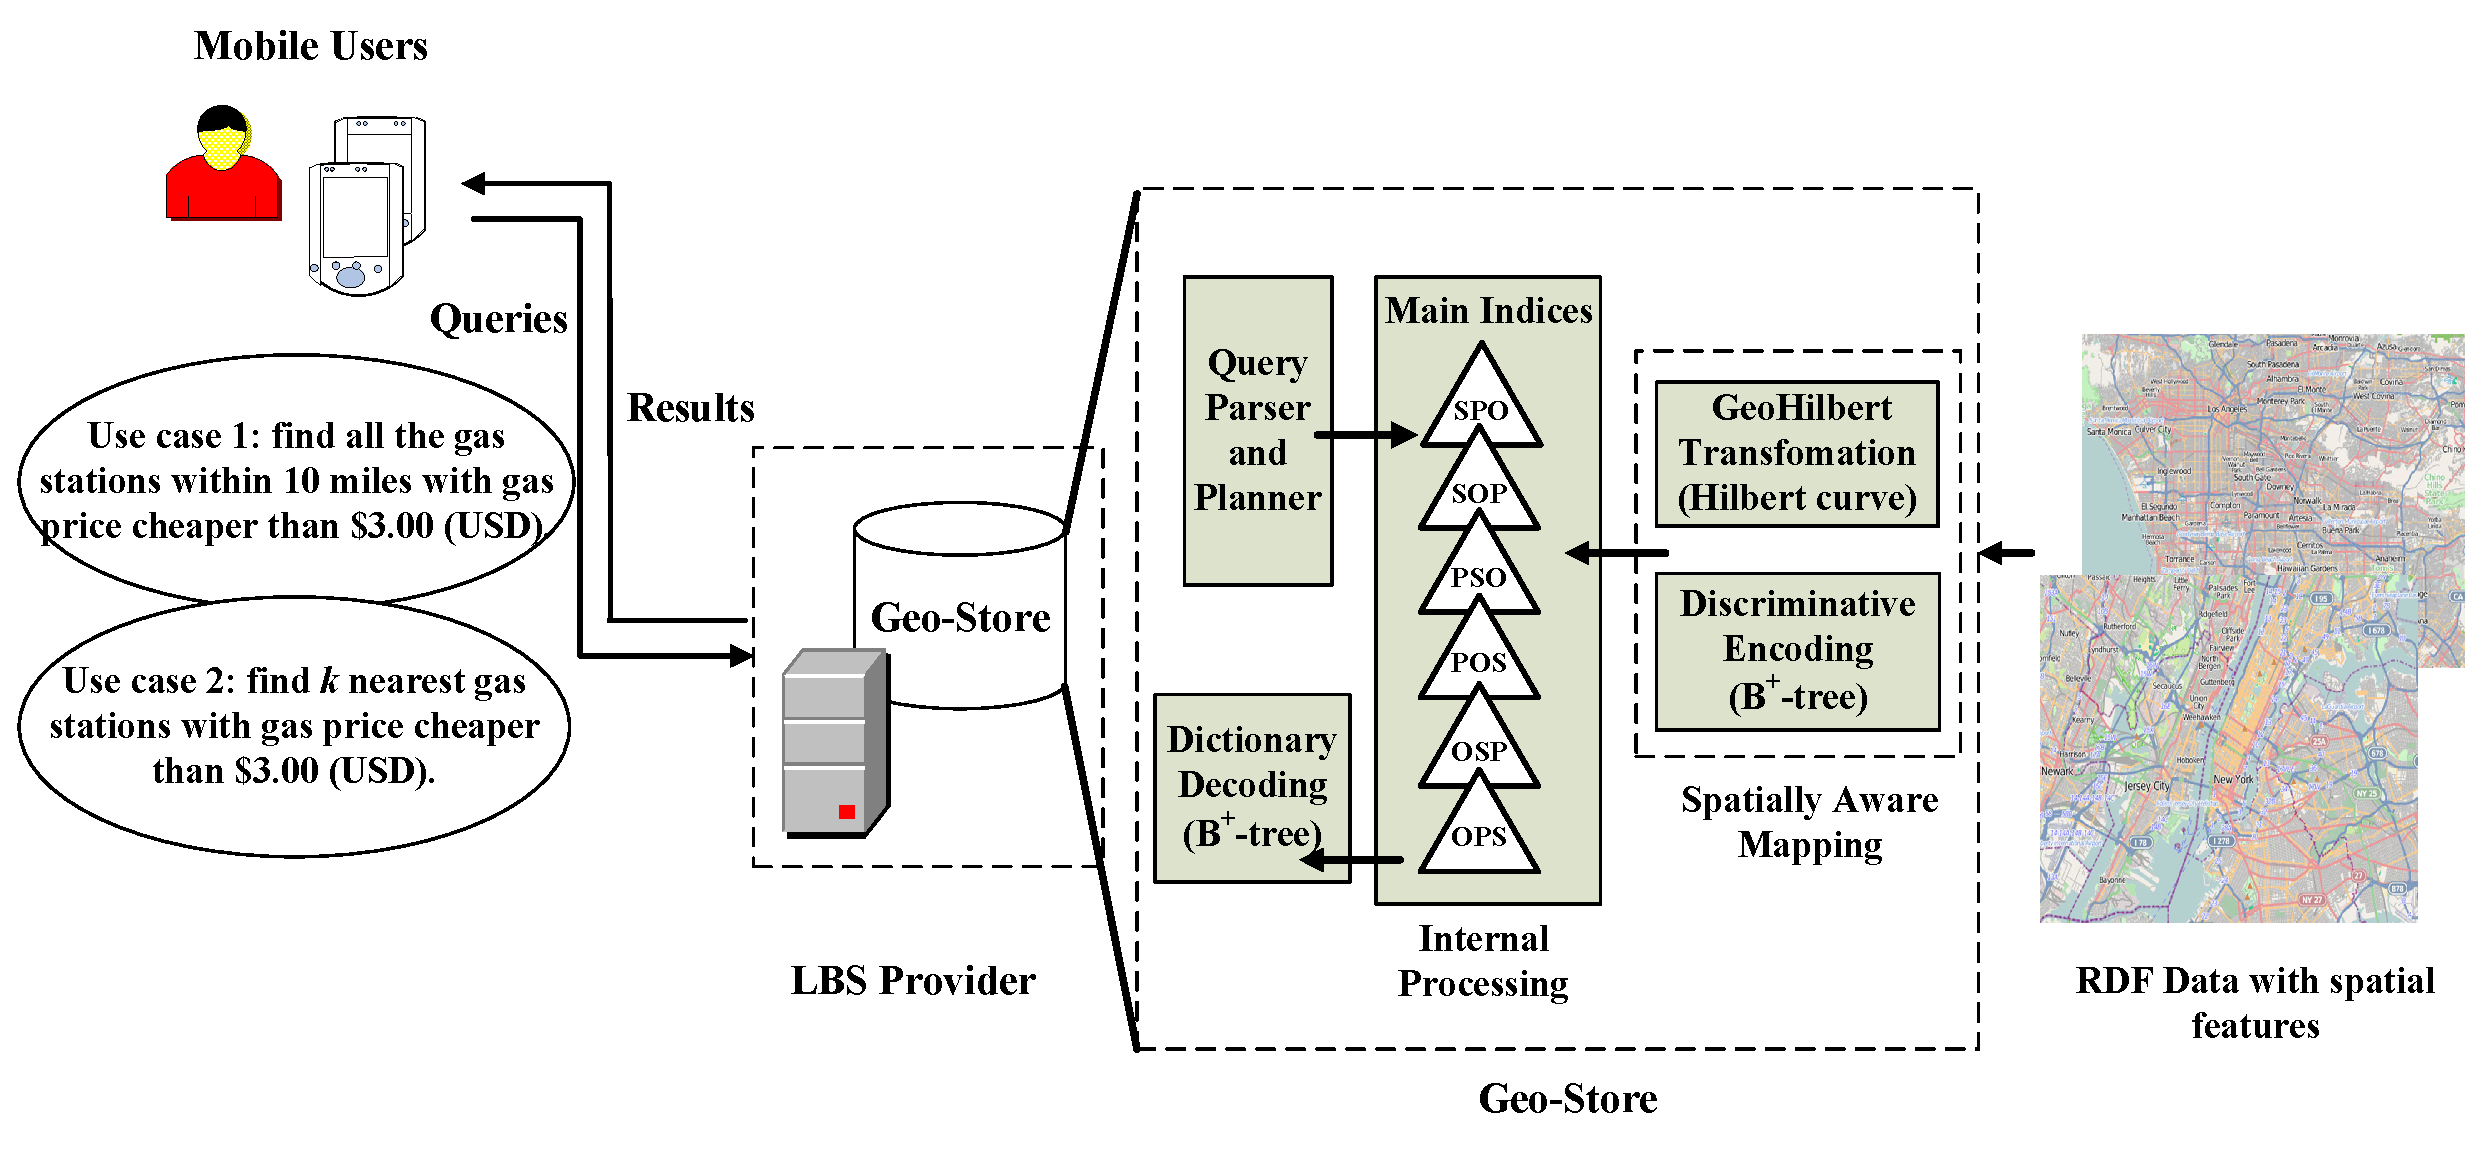
\psfig{file=geo-store-journal/image/framework2.eps,width=6.5in}}
\caption{Geo-Store system architecture and use cases.}
\label{fig-framework} \vspace*{-10pt}
\end{center}
\end{figure*}


\subsubsection{Spatially Aware Mapping Module}

In most of the existing triple stores, each URI or literal is replaced with a unique integer ID by dictionary mapping because the triples may contain very long URIs and string literals. In our system, in order to support efficient spatial query evaluation on triples, we extend the standard dictionary encoding and design a Spatially Aware Mapping (SAM) approach to encode all the URIs and literals, as well as preserve spatial locality. SAM includes two major components, \emph{GeoHilbert Transformation} and \emph{Discriminative Encoding}. With GeoHilbert Transformation, original RDF triples are transformed to the corresponding GeoHilbert representation. In addition, SAM assigns an ID to each URI and literal in a discriminative way in order to maintain spatial locality by executing the discriminative encoding component.

\paragraph{GeoHilbert Transformation}

We utilize a novel RDF representation, GeoHilbert, to model spatial data in Geo-Store. GeoHilbert is designed for incorporating the Hilbert curve-based spatial transformation information into original RDF data. GeoHilbert consists of a subject, \emph{HilbertMapping} and four predicates: \emph{StartPoint}, \emph{Order}, \emph{Orientation}, and \emph{Pos}. Specifically, the values of \emph{StartPoint}, \emph{Order}, \emph{Orientation}, and \emph{Pos} are the location of the Hilbert curve starting point, the curve order $O$, the curve orientation $\theta$, and a Hilbert value translated from a given spatial location, respectively.

Listing~\ref{list4} demonstrates the corresponding RDF data in the
GeoHilbert representation for the restaurant described in
Listing~\ref{list2}. As shown in Listings~\ref{list3}
and~\ref{list4}, the GeoHilbert representation appends to the
original RDF representation an additional RDF statement,
\{\emph{gstore:Point738330640}, \emph{gstore:Pos},
\emph{``208083"}\}, which stores the relative position of the
referred point along the Hilbert space-filling curve.

%\newpage

\begin{lstlisting}[caption={The GeoHilbert representation of the restaurant described in Listing~\ref{list2}.}, label={list4}]
...
gstore:HilbertMapping gstore:StartPoint  "32.3372200 -114.1369000"
gstore:HilbertMapping gstore:Order       "10"
gstore:HilbertMapping gstore:Orientation "Up Left"
...
gstore:Point738330640 gml:amenity "restaurant"
gstore:Point738330640 gml:cuisine "american"
gstore:Point738330640 gml:name    "Colonial Kitchen"
gstore:Point738330640 gml:pos     "34.1135498  -118.1235345"
gstore:Point738330640 gstore:Pos  "208083"
...
\end{lstlisting}


\paragraph{Discriminative Encoding}

The Discriminative Encoding (DE) component takes the GeoHilbert representation based data as the input. For each literal following the predicate \emph{Pos}, DE assigns it a positive ID which is exactly the same as its Hilbert value. For example, in Listing~\ref{list4}, the literal \emph{``208083"} in the triple \{\emph{gstore:Point738330640}, \emph{gstore:Pos}, \emph{``208083"}\} will be assigned with ID \emph{208083}. For all the other literals or URIs, DE acquires a random integer by calling a dictionary encoding function, and then returns the opposite of that integer as the ID (e.g., a randomly generated integer ``1000" will be returned as ``$-$1000"). All the assigned IDs are maintained in a B$^{+}$-tree to speed up the dictionary lookup.

\subsubsection{Internal Processing Module}

Generally, the evaluation of SPARQL queries is based on pattern matching. In this system, we maintain in memory all six possible permutations of \emph{subject} (S), \emph{predicate} (P), and \emph{object} (O) in six separate indices in order to guarantee that every possible query pattern in a SPARQL query with variables in any position of a triple can be answered by only performing a single index scan. Specifically, these permutations are named as SPO, SOP, OSP, OPS, PSO, and POS indices, respectively. Notice that instead of the original URIs or literals, all the six indices here consist of integer IDs, which are assigned by the discriminative encoding component. This ID-based indexing scheme can both save memory space and accelerate join processing.

\subsubsection{Query Parser and Planner Module}

When Geo-Store receives a SPARQL query $q$, it parses $q$, identifies the IDs that have been assigned to the literals in $q$ according to SAM, and employs the retrieved IDs to replace the corresponding literals in $q$. By executing these processes, the subsequent evaluation of $q$ purely relies on the comparisons of IDs instead of the original literals. A query evaluation plan can then be generated accordingly.

\subsubsection{Dictionary Decoding Module}

After the SPARQL query is evaluated by the internal processing module, the dictionary decoding module transforms the resulting IDs back to their original literals as the query results. In Geo-Store, we employ a B$^{+}$-tree structure to implement this ID-to-literal mapping.

\section{Semantics Enabled Location-based Services with Spatial Encoding}\label{sec-query}

The SPARQL query language is standardized by the World Wide Web
Consortium (W3C) for querying RDF data. Evaluation of SPARQL
queries is based on pattern matching on the target RDF graph. A
pattern may contain variables that are bound to a URI or a
literal. In addition, the SPARQL query language provides a number
of built-in FILTER functions, which can be easily extended to
support spatial operations (or constraints). Because range and $k$
nearest neighbor queries are the building blocks of location-based
services, we elaborate on how to evaluate the two important query
types by utilizing our system in this section.


\subsection{Range Queries}


Listing~\ref{list5} shows a sample range query which is launched
to retrieve the latitude and longitude values of all the qualified
gas stations with the two selection conditions: (1) the location
is less than 10 miles away from the query point (the mobile user's
current location), and (2) the gas price is cheaper than \$3.00
per gallon.

%\newpage

\begin{lstlisting}[caption={The sample range query in Geo-Store (use case 1).}, label={list5}]
SELECT ?coordinates
WHERE {
  ?point a "Gas Station" .
  ?point gml:pos ?coordinates .
  FILTER (gstore:range(?point, CURRENT_LOCATION, 10, "mile"))
  ?point gstore:gaspriceUSD ?price .
  FILTER (?price < 3.00)
}
\end{lstlisting}

\begin{figure*}[!h]
\begin{center}
 \begin{tabular}{cc}
 \psfig{figure=geo-store-journal/image/hilbert.eps,height=2.0in}  &
 \psfig{figure=geo-store-journal/image/range_query.eps,height=2.0in}  \\
 \parbox{2.2in}{\centering (a) Hilbert curve transformation.} &
 \parbox{2.2in}{\centering (b) Range query $Q_R$.} \\
 \end{tabular}
 \caption{Hilbert curve transformation and range query.}
 \label{fig-hilbert}
\end{center}
\end{figure*}

In Geo-Store, each spatial object is annotated with its Hilbert
value information based on the GeoHilbert representation.
Figure~\ref{fig-hilbert}(a) illustrates an example of mapping
spatial objects in a two dimensional space into their Hilbert
values. In Figure~\ref{fig-hilbert}(a), the entire space is
divided by the Hilbert curve into 64 grids with their unique
Hilbert values, and we can acquire the Hilbert values of the
spatial objects \emph{A}, \emph{B}, and \emph{C}, as 29, 32, and
7, respectively. Depending on the desired resolution, more
fine-grained curves can be recursively generated based on the
Hilbert curve generation algorithm. Figure~\ref{fig-hilbert}(b)
demonstrates how a range query can be processed in our system by
taking advantage of the Hilbert values of spatial objects. As
depicted in Figure~\ref{fig-hilbert}(b), the query point is
\emph{q} and the query window of the range query $Q_R$,
highlighted in red, covers the three Hilbert curve segments
[10-12], [17-18], and [28-31]. After obtaining the above three
curve segments, our system retrieves all the spatial objects whose
Hilbert values are embraced by the three curve sections and treats
the retrieved spatial object set $\mathbb{R}^{\prime}$ as the
inclusive query result. Subsequently, our system examines all the
spatial objects in the grids that \emph{partially} overlap with
the query window (i.e., grids [10-12], [28] and [31]) to check if
their exact locations (i.e., latitude and longitude values) are
within the query window by dictionary lookup. Finally, the exact
query result $\mathbb{R}$ is returned to the user after filtering
out those objects whose locations are outside the query window in
the partially overlapping grids.


\subsection{$k$ Nearest Neighbor Queries}

In this subsection, we extend our range query solution to evaluate
$k$ nearest neighbor queries efficiently in Geo-Store.
Listing~\ref{list6} demonstrates a sample $k$ nearest neighbor
query which is issued to retrieve the latitude and longitude
values of the gas stations that are among the $k$ closest gas
stations to the query point with a listed gas price cheaper than
\$3.00 per gallon.


%\lstset{showstringspaces=false} \lstset{basicstyle=\ttfamily\small,escapeinside={`}{`}}

\begin{lstlisting}[caption={The sample $k$ nearest neighbor query in Geo-Store (use case 2).}, label={list6}]
SELECT ?coordinates
WHERE {
  ?point a "Gas Station" .
  ?point gml:pos ?coordinates .
  FILTER (gstore:NN(?point, CURRENT_LOCATION, k))
  ?point gstore:gaspriceUSD ?price .
  FILTER (?price < 3.00)
}
\end{lstlisting}

Given a query point $q$, Geo-Store searches the spatial objects in
both the ascending and descending directions of Hilbert values
until $k$ spatial objects are found, and then records the result
set as $\mathbb{S}$. Supposing the object $o$ has the longest
distance to $q$ in $\mathbb{S}$, $Distance(q, o)$ (the distance
between $q$ and $o$) is set as the \emph{search upper bound} for
the subsequent range query. Afterwards, Geo-Store launches a range
query $Q_{R}$ with $Distance(q, o)$ to decide the query window
size and then acquires the query result $\mathbb{R}^{\prime}$.
Next, Geo-Store identifies the top $k$ objects in
$\mathbb{R}^{\prime}$ based on their respective distances to $q$
in order to derive the final query result $\mathbb{R}$.

Figure~\ref{fig-NN} demonstrates the evaluation of a $k$ nearest
neighbor query with Geo-Store. As shown in Figure~\ref{fig-NN}(a),
based on the query point $q$, Geo-Store first searches for spatial
objects with Hilbert values $\geq 30$ and $< 30$ in parallel until
$k$ objects are discovered. Next, assume that the spatial object
that has the longest distance to $q$ among the above $k$ objects
is object $B$. Then, a range query $Q_R$ with the distance between
$q$ and $B$ as the search upper bound is issued; $Q_R$ returns the
result set $\mathbb{R}^{\prime}$, as depicted in
Figure~\ref{fig-NN}(b). In this example, set $\mathbb{R}^{\prime}$
encompasses objects which fall on the five Hilbert curve segments,
[8-20], [23-24], [27-32], [35-36], and [53-54]. Finally, Geo-Store
computes the top $k$ objects in $\mathbb{R}^{\prime}$ with the
shortest distance to $q$ as the exact query result.

\begin{figure*}[!h]
\begin{center}
 \begin{tabular}{cc}
 \psfig{figure=geo-store-journal/image/NN_search.eps,height=2.0in}  &
 \psfig{figure=geo-store-journal/image/NN.eps,height=2.0in}  \\
 \parbox{2.3in}{\centering (a) Finding the search upper bound.} &
 \parbox{2.3in}{\centering (b) The derived range query $Q_{R}$.}
 \end{tabular}
 \caption{$k$ nearest neighbor query example.}
 \label{fig-NN}
\end{center}
\end{figure*}


\section{Experimental Validation}\label{sec-experiment}

For performance evaluation, we compared our Geo-Store system with
Brodt's system~\cite{conf/gis/BrodtNM10} and the Strabon
system~\cite{KyzirakosKK10} by measuring their response time on
processing two popular location-based spatial query types, range
and $k$NN. We acquired the locations of points of interest (POI)
in California from the U.S. Geological
Survey\footnote{http://cumulus.cr.usgs.gov/}. This real-world data
set contains one million POIs distributed over the state of
California with 63 different POI categories, including airport,
hospital, school, populated place, road junction, etc. Each
category exhibits a distinct density and distribution. For each
result in this section, we ran $500$ corresponding queries with
distinct query points whose locations were randomly generated
within the state of California. All the experiments were conducted
on the same Windows machine.

%We measured the end-to-end execution time (response time) by
%counting from the time of query submission to the time returning
%the final results to mobile users.

\subsection{Efficiency Comparison}

In this subsection, we focus on comparing the efficiency of
Geo-Store, Brodt's, and Strabon in terms of query response time.

\subsubsection{Range query}

We first report our experimental results of range queries. We
gradually increased the area of the query window to investigate
its impact on query response time. Here we specify the area of a
query window by using the percentage of the region of California.
For example, a query window with the percentage of 0.01\%
represents an area of around 16 square miles (given the region of
California is around 160,000 square miles). As shown in
Figure~\ref{fig-result} (a), with the enlargement of the query
window, the response time kept increasing for all systems.
However, our Geo-Store system always outperformed Brodt's and
Strabon. For instance, with the query window of 0.01\%, Geo-Store
only required 0.422 seconds on average to execute the range query,
while Brodt's and Strabon needed 1.916 seconds and 2.792 seconds,
respectively. The advantage of Geo-Store over the other two
systems, in terms of efficiency in evaluating range queries, can
be explained as follows.

By utilizing the Hilbert curve based transformation, Geo-Store
manages to maintain a roughly one-to-one mapping between Hilbert
values and POIs. Therefore, in most cases, the spatial relation
between two entities can be determined by comparing their
respective Hilbert values. As a result, if a POI is identified as
beyond the query window by the examination of its Hilbert value,
it can be filtered out at an earlier stage, and there will be no
need to check its exact latitude/longitude information on disk. On
the contrary, in Brodt's and Strabon (both employ the R-tree
index), each Minimum Bounding Rectangle (MBR) contains numerous
POIs (i.e., usually more than half of the fan-out value),
resulting in a much larger amount of I/Os to retrieve the
latitude/longitude values on disk in order to decide if a
particular POI satisfies a spatial selection operation or not.

\subsubsection{$k$ nearest neighbor query}

Next we study the efficiency of all three systems in evaluating
$k$ nearest neighbor queries. We varied the $k$ value from 1 to
10. Figure~\ref{fig-result} (b) shows that when we elevated the
$k$ value, all the systems required a longer response time to
identify the $k$ closest neighbors. Nevertheless, as demonstrated
in Figure~\ref{fig-result} (b), the response time needed by
Geo-Store was significantly reduced, compared to the other two
systems. For example, with $k$ equal to 3, Geo-Store only required
0.325 seconds on average, while Brodt's and Strabon needed 0.913
seconds and 1.642 seconds, respectively. Geo-Store demonstrates a
much higher efficiency than the other two systems in processing
$k$ nearest neighbor queries because Hilbert values employed in
Geo-Store can provide a more precise location estimation of each
POI than MBRs used in R-trees, which improves query evaluation
performance.


\begin{figure*}[!h]
\begin{center}
 \begin{tabular}{cc}
 \psfig{figure=geo-store-journal/image/rq_result.eps,height=2.0in}  &
 \psfig{figure=geo-store-journal/image/nn_result.eps,height=2.0in}  \\
 \parbox{2.0in}{\centering (a) Range query.} &
 \parbox{2.0in}{\centering (b) $k$ nearest neighbor query.} \\
 \end{tabular}
 \caption{Performance comparison of the three systems.}
 \label{fig-result}
\end{center}
\end{figure*}


%\subsection{Scalability Comparison}

%Here we investigated the performance of Geo-Store and the R-tree
%solution with regard to scalability by varying \emph{the total
%number of POIs} from 10K, 20K, 50K, to 100K.

%\subsubsection{Range query}

%Figure~\ref{fig-sca} (a)


%\subsubsection{$k$ nearest neighbor query}

%Figure~\ref{fig-sca} (b)


\subsection{Integration with Existing Triple Stores}

As discussed in Section~\ref{sec-design}, one of the clear
advantages that Geo-Store provides over Brodt's solution is that
no complicated spatial index, such as an R-tree, is needed to be
maintained in Geo-Store. The indexing mechanism in Geo-Store is
completely consistent to the six separate indices
design~\cite{journals/pvldb/WeissKB08}, which is employed in most
existing triple
stores~\cite{conf/www/CarrollDDRSW04,conf/vldb/AbadiMMH07,journals/pvldb/WeissKB08,journals/vldb/NeumannW10}
for RDF query evaluation. On the other hand,
in~\cite{conf/gis/BrodtNM10}, a separate R-tree is responsible for
indexing all the spatial IDs while all the IDs, spatial or
non-spatial, are indexed by a B$^{+}$-tree. Therefore, by using
our design, current RDF triple stores can be easily extended to
support location-based services with limited cost on integration.


%section{Conclusions}\label{sec-conc}
%The increasing amount of RDF data containing location-based information calls for the development of systems which support effective evaluation of location-based services on RDF triple stores. In our Geo-Store project, we implement a system which is capable of querying heterogenous data sources and providing semantics-enabled location-based services with high efficiency. The Geo-Store system confers the following advantages. First, Geo-Store utilizes Spatially Aware Mapping to preserve spatial locality during encoding. Second, as our experiments demonstrate, Geo-Store allows for effective processing of range and $k$NN queries. Third, existing triple stores can be easily integrated with Geo-Store with limited integration cost.

For future work, we plan to extend Geo-Store to support other novel RDF query languages specifically designed for spatial data management, such as GeoSPARQL and stSPARQL, by expanding the query parser module and related components. In addition, we will support more spatial query types, such as spatial join, in the next phase of this project.


%(such as map data or sensor data)



%\chapter{Tasks and Schedule}

\section{Tasks}

\subsection{Hierarchical Data in Relational Database Management Systems}

For our work on hierarchical date index, we have already explored related works, and studied the theoretical background that supports our design. In additional to the work we have done, the following are the work still to be done.

\begin{enumerate}
\item Design experiments to evaluate the efficiency of our design.
\item Implement experiments.
\item Report experimental results and finalize paper.
\end{enumerate}


\subsection{Efficient Evaluation of Skyline Queries}

For this work, we are exploring a new algorithm for evaluating skyline operations. Specifically we are exploring an algorithm based on the Branch and Bound Skyline (BBS). With out algorithm, we aim to improve the memory and the speed over BBS. The following are the task items.

\begin{enumerate}
\item Research into new skyline algorithm.
\item Design and conduct experiments.
\item Report experimental results.
\end{enumerate}

\subsection{Moving Toward Semantic Web Database}

The follow are the task items.

\begin{enumerate}
\item Study benefit of using semantic web technology.
\item Alternatives to semantic web.
\item Design experimental database.
\item Report results.
\end{enumerate}

\section{Schedule}

\begin{table}[ht]
\centering
\begin{tabular}{|l|l|l|}
\hline
{\bf Tasks} & {\bf Duration} & {\bf Completion Date} \\ \hline\hline
Research Proposal Defense & 4 weeks & July 31, 2013 \\
Experimental evaluation for hierarchical data index & 4 weeks & August 31, 2013 \\
Finalize hierarchical index design & 2 weeks & September 16, 2013\\
Finalize report for hierarchical index & 2 weeks & September 30, 2013\\
Design experiment and evaluation & 8 weeks & November 30, 2013 \\
Study semantic web and RDF technology & 4 weeks & December 31, 2013\\
Design Experiment and RDF database & 8 weeks & February 28, 2014\\
Design evaluation & 4 weeks & March 31, 2014\\
Finalize dissertation & 8 weeks & May 2014\\
\hline
\end{tabular}
%\caption{Common operation Examples\label{table:common_operation_examples}}
\end{table}

%\bibliographystyle{plain}
%\bibliography{mdpx/ref}


\bibliographystyle{plain}
\bibliography{mdpx/bib/ref,mdpx/bib/cmod,mdpx/bib/mdsplus,mdpx/bib/d3d,mdpx/bib/lhd,mdpx/bib/nstx,mdpx/bib/w7x,mdpx/bib/iter,mdpx/bib/demo,mdpx/bib/epics,bib,mongodb/bib}
\end{document}

